%%  Copyright (c) 2015, 2016, 2017, Intel Corporation
%%  All rights reserved
%%  No license (express or implied, by estoppel or otherwise) to any
%%  intellectual property rights is granted by this document.
%%
\documentclass[11pt]{article}
\usepackage[pdftex]{graphicx}
\usepackage{float}
\usepackage{fullpage}

\usepackage{url}
\usepackage{setspace}

\newcommand{\intel}{Intel\textsuperscript{\textregistered}\ }
\newcommand{\xeonphi}{Intel\textsuperscript{\textregistered} Xeon Phi\textsuperscript{\texttrademark} coprocessor\ }
\newcommand{\xeon}{Intel\textsuperscript{\textregistered} Xeon\textsuperscript{\textregistered} processor\ }
\newcommand{\brand}{\textsuperscript{*}\ }

\begin{document}
\sloppy
\title{GEOPM Plugin Developer's Guide}
\author{Steve Sylvester\\
        Intel Corporation\\
        \small{steve.s.sylvester@intel.com}}
\maketitle
\begin{abstract}
Global Extensible Open Power Manager (GEOPM) is an extensible
power management framework targeting high performance computing. The
library can be extended to support new control algorithms and new
hardware power management features. The GEOPM package provides built
in features ranging from static management of power policy for each
individual compute node, to dynamic coordination of power policy and
performance across all of the compute nodes hosting one MPI job on a
portion of a distributed computing system. The dynamic coordination is
implemented as a hierarchical control system for scalable
communication and decentralized control. This document concentrates on
the development of custom plugins for new control algorithms as well
as new hardware platforms or new power management features.
\end{abstract}

\section{Implementing new control algorithms}
GEOPM supports two levels of control algorithms; A leaf control
algorithm that manages power within a single node, and a tree control
algorithm that manages power between nodes. Internally these are known
as tree deciders and leaf deciders.

\section{Leaf Deciders}
\begin{figure} [H]
  \centering
  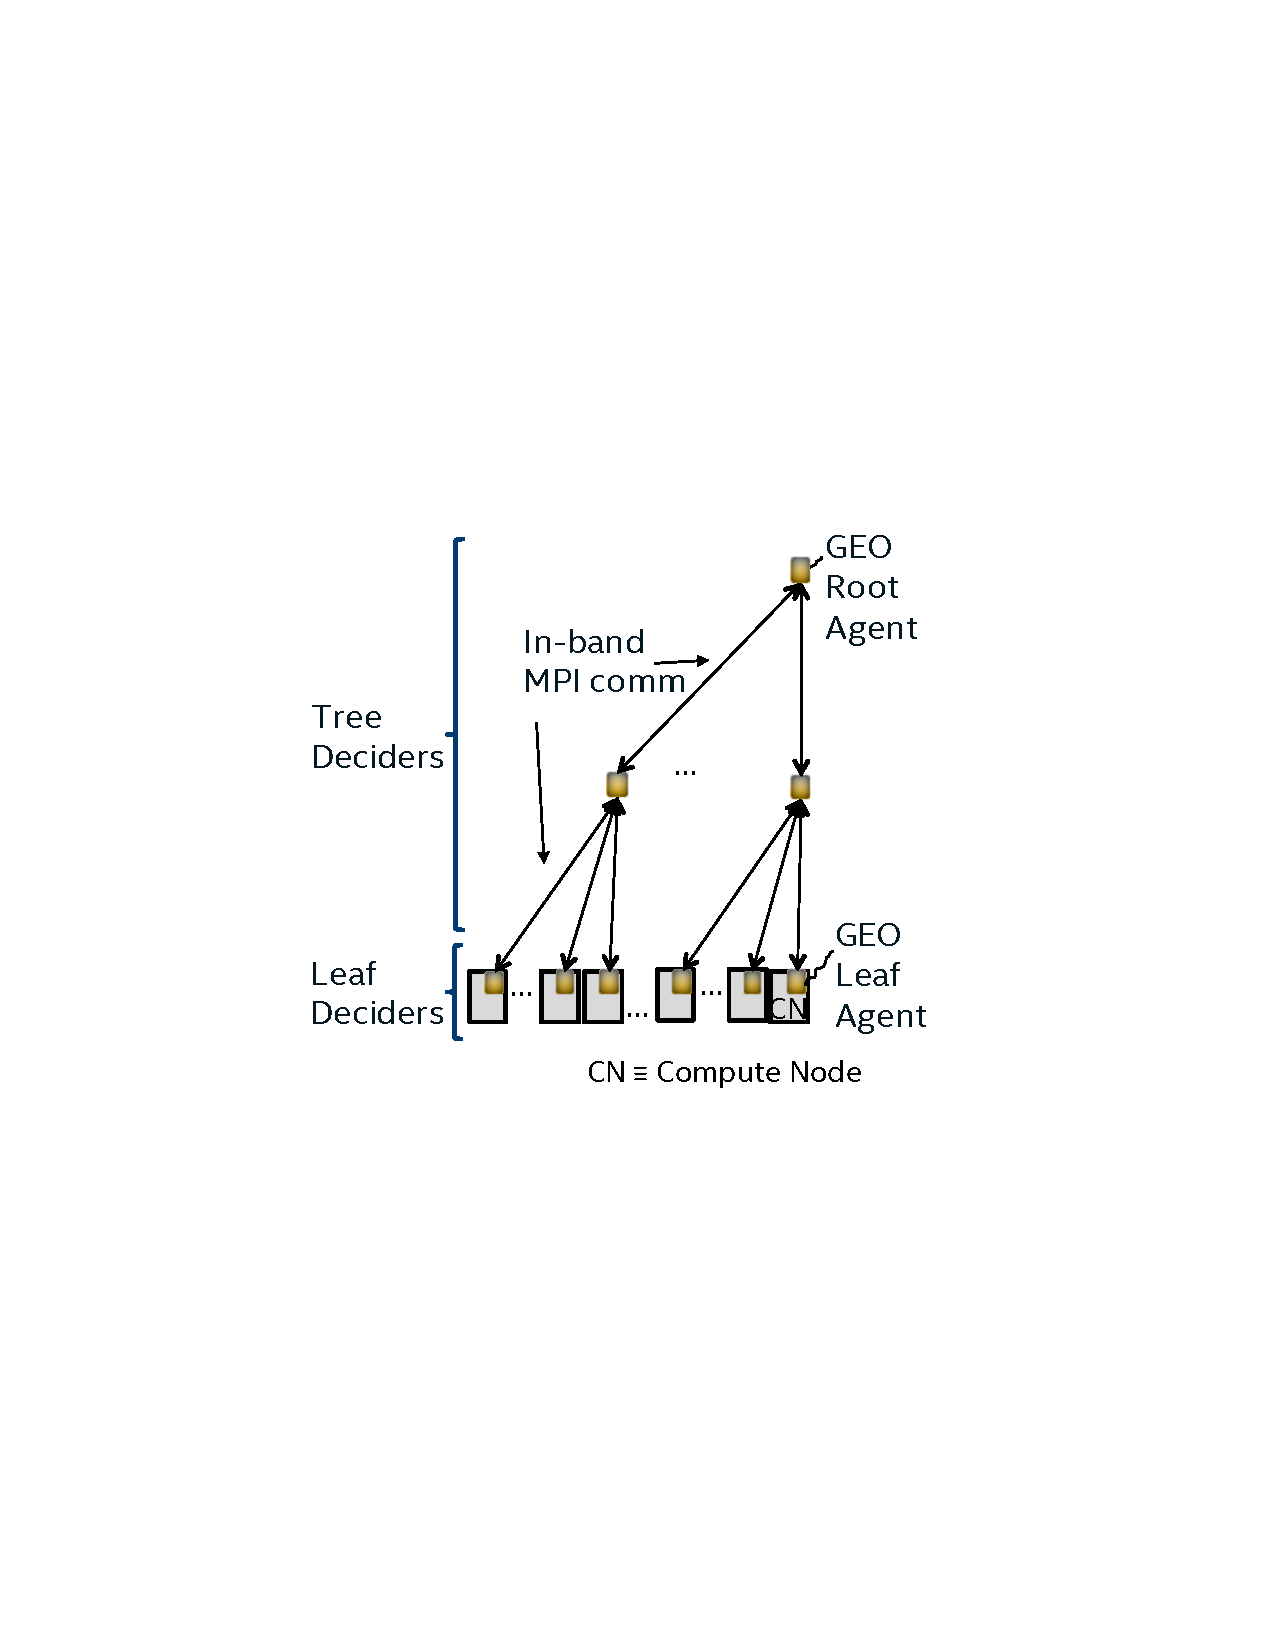
\includegraphics[width=0.5\textwidth]{leaf-figure}
  \caption{Leaf decider data collection}
  \label{fig:leaf}
\end{figure}

As seen if figure \ref{fig:leaf}, event counters and energy meters are
collected from the platform and application data such as runtime and
progress are collected from the individual application ranks on the
node. This data is aggregated for each application region, where a
region is a subset of the application runtime that has uniform
computation characteristics. These characteristics include how compute
bound, memory bound, or network bound the region is. The leaf decider
makes power decisions on a region by region basis. The leaf decider
then uses this data to set new power policies for the domains of
control on the particular hardware platform. For example, If the
method of control is power capping then the domain of control would be
the finest granularity hardware component with RAPL power
controls. For current Xeon platforms based on Haswell, that would be
at the socket level. If the method of control is frequency, then on
current Xeon platforms based on Haswell, that would be at the CPU
level. This data is abstracted away from the decider. It merely has
per domain of control statistics the it can use to set a power policy
for the same set of domains. The current set of signals available to
the leaf decider are captured in the \verb#geopm_telemetry_type_e#
enumeration:

\begin{verbatim}
    enum geopm_telemetry_type_e {
        GEOPM_TELEMETRY_TYPE_PKG_ENERGY,
        GEOPM_TELEMETRY_TYPE_PP0_ENERGY,
        GEOPM_TELEMETRY_TYPE_DRAM_ENERGY,
        GEOPM_TELEMETRY_TYPE_FREQUENCY,
        GEOPM_TELEMETRY_TYPE_INST_RETIRED,
        GEOPM_TELEMETRY_TYPE_CLK_UNHALTED_CORE,
        GEOPM_TELEMETRY_TYPE_CLK_UNHALTED_REF,
        GEOPM_TELEMETRY_TYPE_LLC_VICTIMS,
        GEOPM_TELEMETRY_TYPE_PROGRESS,
        GEOPM_TELEMETRY_TYPE_RUNTIME,
        GEOPM_NUM_TELEMETRY_TYPE // Signal counter, must be last
    };
\end{verbatim}

\section{Tree Deciders}
\begin{figure} [H]
  \centering
  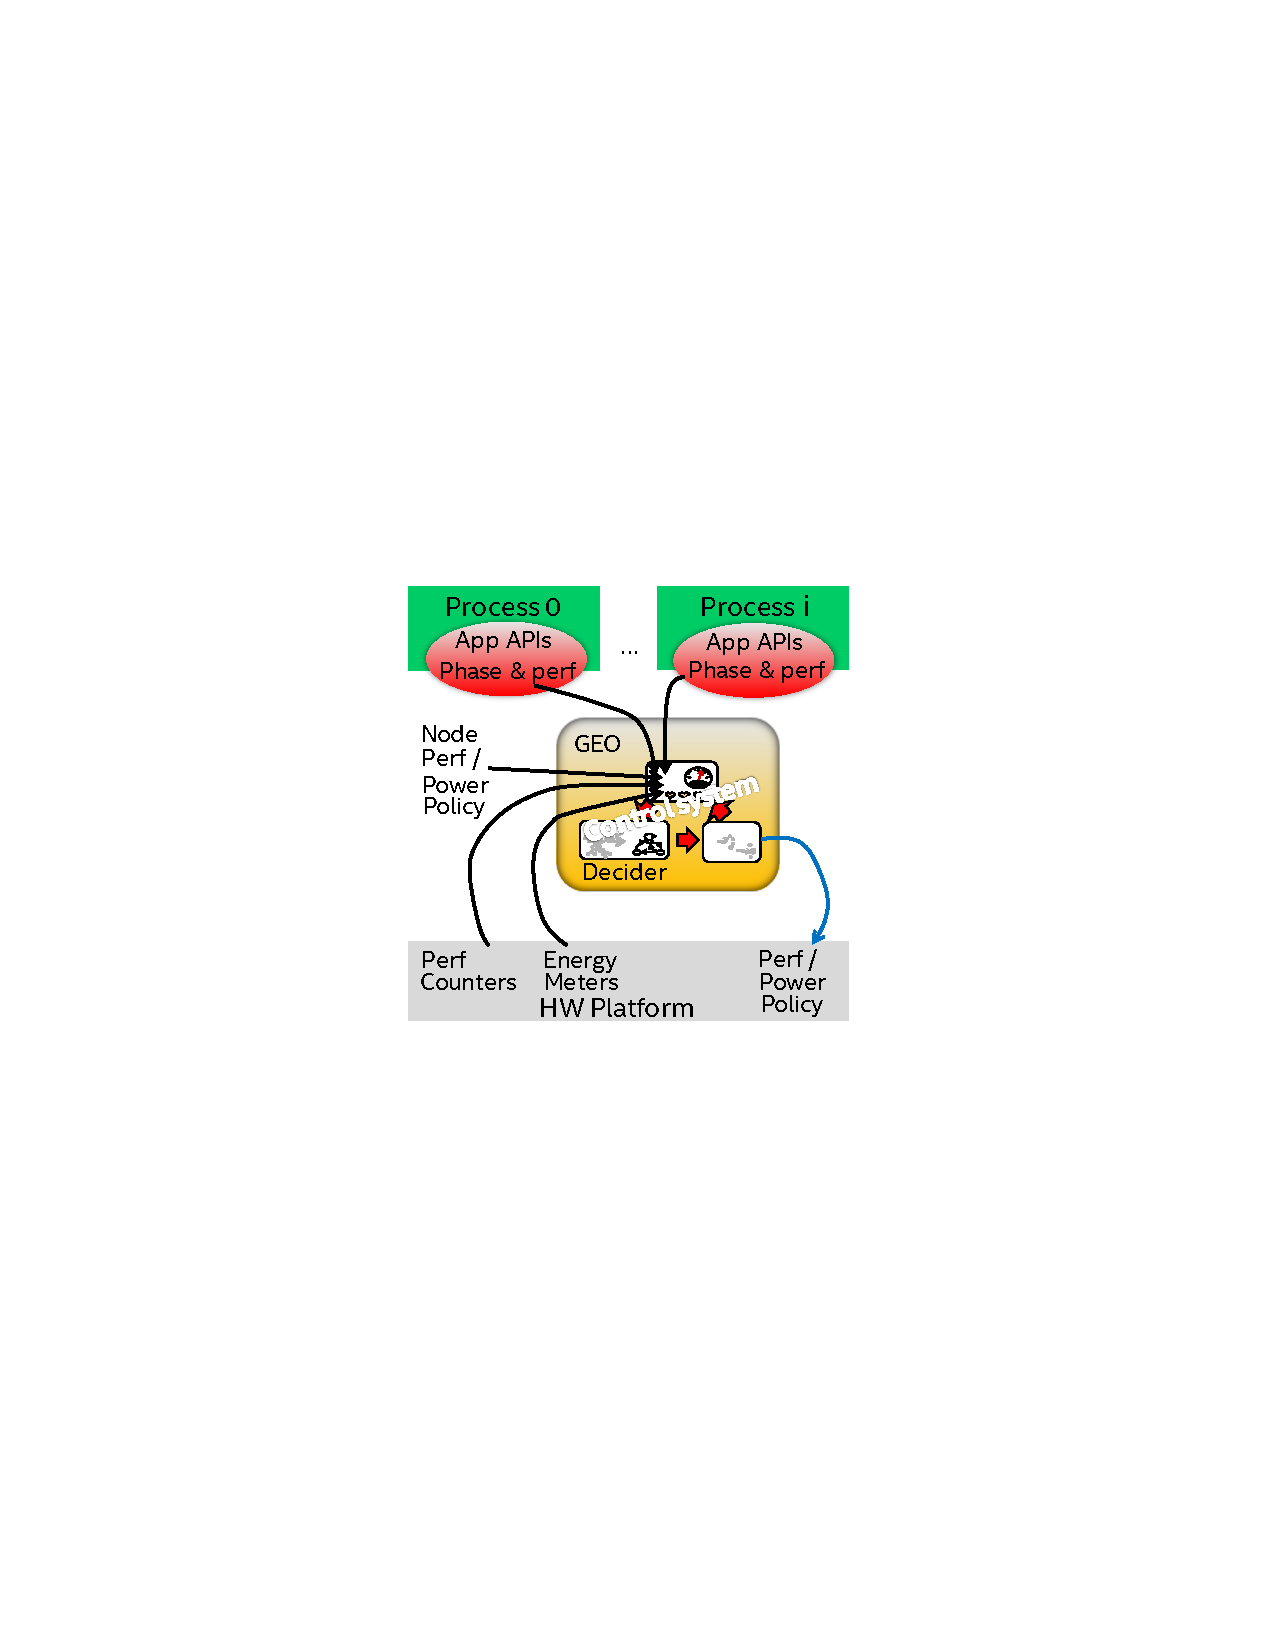
\includegraphics[width=0.5\textwidth]{tree-figure}
  \caption{Data collection andn power budget flow at the tree level}
  \label{fig:tree}
\end{figure}

At the tree level, as can be seen in figure \ref{fig:tree}, The domain
of control is always the number of nodes which are direct children of
the node in question. Data at the leaf level is aggregated and sent up
the tree to the parent. That parent and it’s siblings have tree
deciders which use the aggregated data to create and send power
budgets back down to the leaf nodes. The parent and it’s sibling also
aggregate their data and send it up to the next level of the tree
where the same thing happens. This continues all the way to the root
of the tree. At any point in the tree the power budget is the
aggregated budget for all leaf nodes in the nodes subtree. The current
set of signals available to the leaf decider are captured in the
\verb#geopm_sample_type_e# enumeration:

\begin{verbatim}
    enum geopm_sample_type_e {
        GEOPM_SAMPLE_TYPE_RUNTIME,
        GEOPM_SAMPLE_TYPE_ENERGY,
        GEOPM_SAMPLE_TYPE_FREQUENCY,
        GEOPM_NUM_SAMPLE_TYPE // Sample counter, must be last
    };
\end{verbatim}

\section{Plugin Registration}
Every plugin must export a C function that allows the plugin to
register itself with the GEO runtime.

\begin{verbatim}
    int geopm_plugin_register(int plugin_type, struct geopm_factory_c *factory)
    {
        int err = 0;
        try {
            if (plugin_type == GEOPM_PLUGIN_TYPE_DECIDER) {
                geopm::Decider *decider = new geopm::CustomDecider;
                geopm_factory_register(factory, decider);
            }
        }
        catch(...) {
             err = geopm::exception_handler(std::current_exception());
        }
        return err;
    }
\end{verbatim}
The function checks if it is the type being looked for, and if it is,
it creates an instance itself and registers it with the passed in
factory. In this example the plugin class is called
\verb#CustomDecider#.

\section{Extending geopm::Decider base class}
The \verb#geopm:Decider# class has a number of pure virtual methods
that must be overridden by the derived plugin class.
\begin{verbatim}
    virtual Decider *clone() const = 0;
    virtual const std::string& name(void) const = 0;
    virtual bool decider_supported(const std::string &descripton) = 0;
    virtual bool update_policy(Region &curr_region, Policy &curr_policy) = 0;
\end{verbatim}
The \verb#clone# method simply returns a copy of an instance of the
class. This is for the internal use of the geopm runtime.
\begin{verbatim}
    Decider *CustomDecider::clone(void) const
    {
        return (Decider*)(new CustomDecider(*this));
    }
\end{verbatim}
A string description should be created for each plugin. The string
should be unique among all decider plugins. If not unique then the
first instance will be chosen at runtime. Some examples are:
\begin{verbatim}
    const std::string m_name("powerbalancing");
\end{verbatim}
or
\begin{verbatim}
    const std::string m_name("powergoverning");
\end{verbatim}
The name function simply returns the string description of the custom
decider.
\begin{verbatim}
    const std::string& CustomDecider::name(void) const
    {
        return m_name;
    }
\end{verbatim}
The \verb#decider_supported# method is the mechanism used by the
runtime to choose a specific decider. It is simply a check against the
string description of the plugin.
\begin{verbatim}
    bool CustomDecider::decider_supported(const std::string &description)
    {
        return (description == m_name);
    }
\end{verbatim}
The \verb#update_policy# method is where the custom control algorithm
is implemented. It takes in a \verb#Region# object which holds the
telemetry data for the current region as well as a \verb#Policy#
object which holds the current policy for all regions at this level of
the tree. The \verb#Region# object can be queried for telemetry for
each domain of control through the following methods:
\begin{verbatim}
    double signal(int domain_idx, int signal_type);
    int num_sample(int domain_idx, int signal_type) const;
    double mean(int domain_idx, int signal_type) const;
    double median(int domain_idx, int signal_type) const;
    double std_deviation(int domain_idx, int signal_type) const;
    double min(int domain_idx, int signal_type) const;
    double max(int domain_idx, int signal_type) const;
    double derivative(int domain_idx, int signal_type) const;
\end{verbatim}
All of these APIs take in a domain index, where the total number of
domains can be queried from the \verb#Policy# object. The second
parameter is the signal type on which to operate. At the leaf they are
\verb#geopm_telemetry_type_e# enums and for the tree that are
\verb#geopm_sample_type_e enums#.  The signal function returns the
last recorded value of the requested signal type.  The
\verb#num_sample# returns the number of samples used to calculate the
values returned by the rest of the functions.  The rest of the
functions return the statistical value described by the function name
over some number of samples.  As a leaf level example, to get the
derivative of package power over the first domain of control:
\begin{verbatim}
    bool CustomDecider::update_policy(Region &curr_region, Policy &curr_policy)
    {
        int first_domain_index = 0;
        double pkg_power = curr_region.derivative(first_domain_index,
                                                  GEOPM_TELEMETRY_TYPE_PKG_ENERGY);
    . . .
\end{verbatim}
At the tree level, to get the maximum runtime for the first domain of
control:
\begin{verbatim}
    bool CustomDecider::update_policy(Region &curr_region, Policy &curr_policy)
    {
        int first_domain_index = 0;
        double max_runtime = curr_region.max(first_domain_index,
                                             GEOPM_SAMPLE_TYPE_RUNTIME);
    . . .
\end{verbatim}
After the statistics are used to calculate new power budgets or
frequencies for each domain of control, the new budgets are applied to
the policy object using either of the APIs:
\begin{verbatim}
    void update(uint64_t region_id, int domain_idx, double target);
    void update(uint64_t region_id, const std::vector<double> &target);
\end{verbatim}
The \verb#update_policy# function should return true if the policy was
modified for any domain of control and false if no modifications were
made. This signals the geopm runtime to apply the new budgets.  When
the algorithm reaches a state when it has figured out the best policy
for the current region for the current power budget, the decider must
mark the region as converged. This lets the geopm runtime know that it
may send aggregated sample data up the tree to the parent, whom then
may send an updated power budget back down. This is done using the
\verb#Policy# object API:
\begin{verbatim}
    void is_converged(uint64_t region_id, bool converged_state);
\end{verbatim}
There is one more API that is not pure virtual but can be overridden
by the plugin:
\begin{verbatim}
    virtual bool update_policy(const struct geopm_policy_message_s &policy_msg,
                               Policy &curr_policy);
\end{verbatim}
It is similar to the pure virtual \verb#update_policy#, except that it
takes in a \verb#geopm_policy_message_s# structure instead of a Region
object. The function gets called by the geopm runtime when it receives
a new power policy message from its parent. At the root of the tree
the parent would be a power aware scheduler/resource manager. The
default implementation simply splits the new budget evenly among all
the domains of control, however different deciders could implement
different methods of splitting the budget. One example is to split the
new budget by the same ratios the current budget was split among the
domains of control. Just like the previous \verb#update_policy#
function, it is expected that the function returns true if a policy is
modified for any domain of control and false if no policies are
modified. The budget in the \verb#geopm_policy_message_s# structure is
the total budget for all domains of control. It should be saved off as
state for use in the pure virtual version of \verb#update_policy#.

\section{Implementing new platform plugins}
The geopm package can be extended to run on new hardware platforms or
support new power management features by creating \verb#Platform# and
\verb#PlatformImp# plugins. A \verb#PlatformImp# plugin implements the
fine details of a specific hardware platform. In the case of an Intel
platform, it encodes things such as the offsets of certain model
specific registers, as well as the topology and capabilities of that
platform. A \verb#Platform# plugin is an abstraction of the
\verb#PlatformImp# interface and is focused on methods of control that
may be supported by many different \verb#PlatformImp# objects. As an
example geopm has a built-in \verb#RAPLPlatform# object which
abstracts the power limiting functionality of Running Average Power
Limiting (RAPL) functionality as well as performance counter access
across may different hardware platforms. The \verb#PlatformImp#
objects built in to geopm include \verb#IVTPlatformImp# which supports
Sandy Bridge and Ivy Town based Xeon systems and a
\verb#HSXPlatformImp# that supports Haswell based Xeon systems. From
the other perspective a \verb#FreqPlatform# plugin could be created
that modifies frequencies instead of RAPL power. It could use the same
\verb#PlatformImp# objects as the \verb#RAPLPlatform# class without
modifying them.

\section{Plugin Registration}
The plugin registration for a \verb#Platform# or \verb#PlatformImp# is
similar to the \verb#Decider# version. In fact you can implement
several plugins within the same file and have a single registration
function:
\begin{verbatim}
    int geopm_plugin_register(int plugin_type, struct geopm_factory_c *factory)
    {
        int err = 0;
        Decider *decider = NULL;
        Platform *platform = NULL;
        PlatformImp *platform_imp = NULL;
        try {
            switch (plugin_type) {
                case GEOPM_PLUGIN_TYPE_DECIDER:
                    decider = new CustomDecider;
                    geopm_factory_register(factory, decider);
                    break;
                case GEOPM_PLUGIN_TYPE_PLATFORM:
                    platform = new CustomPlatform;
                    geopm_factory_register(factory, platform);
                    break;
                case GEOPM_PLUGIN_TYPE_PLATFORM_IMP:
                    platform_imp = new CustomPlatformImp;
                    geopm_factory_register(factory, platform_imp);
                    break;
            }
        }
        catch(...) {
            err = exception_handler(std::current_exception());
        }
        return err;
    }
\end{verbatim}

\section{Extending geopm::Platform base class}
To extend the \verb#geopm::Platform# class, you must override the
following pure virtual functions:
\begin{verbatim}
    virtual  bool model_supported(int platform_id, const std::string &description)
    const =  0;
    virtual  size_t capacity(void) = 0;
    virtual  void sample(std::vector<struct geopm_msr_message_s> &msr_values) = 0;
    virtual  void enforce_policy(uint64_t region_id, Policy &policy) const = 0;
\end{verbatim}
The \verb#model_supported# function is the mechanism used by the
runtime to choose a specific platform. A hardware identifier id as
well as a description string are passed in by the runtime.  The plugin
uses these as well as any other available information in order to
decide if it sufficiently supports the requested functionality as well
as the underlying hardware. The geopm runtime uses the cpuid
instruction to get the hardware platform ID and sends it in as the
first parameter. The passed in description string comes from the
global power policy. For example the built in \verb#RAPLPlatform#
class is implemented as follows:
\begin{verbatim}
    const int M_SNB_ID = 0x62D; // SandyBridge E
    const int M_IVT_ID = 0x63E; // IvyTown E
    const int M_HSX_ID = 0x63F; // Haswell E
    const std::string m_description(“rapl”);
    bool RAPLPlatform::model_supported(int platform_id,
                                       const std::string
                                       &description) const
    {
        return ((platform_id == M_IVT_ID ||
                 platform_id == M_SNB_ID ||
                 platform_id == M_HSX_ID) &&
                description == m_description);
    }
\end{verbatim}
The \verb#capacity# method returns the number of signals that will be
returned when the sample method is called. This lets the caller
pre-size the vector that will hold the data. For the
\verb#RAPLPlatform# it returns 3 signals per socket and 4 signals per
cpu and is implemented as follows:
\begin{verbatim}
    size_t RAPLPlatform::capacity(void)
    {
          return m_imp->num_package() * m_imp->num_package_signal() +
                   m_imp->num_logical_cpu() * m_imp->num_cpu_signal();
    }
\end{verbatim}
The \verb#m_imp# is a pointer to a \verb#PlatformImp# instance which
abstracts the specifics of the underlying hardware.  The \verb#sample#
method takes in a pre-sized vector and fills it with sampled data. It
gets the samples from the \verb#PlatformImp# object that knows how to
query the hardware. It uses the following API from the PlatformImp
object:
\begin{verbatim}
    double read_signal(int device_type, int device_index, int signal_type);
\end{verbatim}
Filling in values for package, dram, and power plane 0 energy on all
sockets:
\begin{verbatim}
    void RAPLPlatform::sample(std::vector<struct geopm_msr_message_s> &msr_values)
    {
        int count = 0;
        struct geopm_time_s time;
        geopm_time(&time);
        //record per package energy readings
        for (int i = 0; i < m_num_package; i++) {
            msr_values[count].domain_type = GEOPM_DOMAIN_PACKAGE;
            msr_values[count].domain_index = i;
            msr_values[count].timestamp = time;
            msr_values[count].signal_type = GEOPM_TELEMETRY_TYPE_PKG_ENERGY;
            msr_values[count].signal =
                m_imp->read_signal(GEOPM_DOMAIN_PACKAGE, i,
                                   GEOPM_TELEMETRY_TYPE_PKG_ENERGY);
            count++;
            msr_values[count].domain_type = GEOPM_DOMAIN_PACKAGE;
            msr_values[count].domain_index = i;
            msr_values[count].timestamp = time;
            msr_values[count].signal_type = GEOPM_TELEMETRY_TYPE_PP0_ENERGY;
            msr_values[count].signal =
            m_imp->read_signal(GEOPM_DOMAIN_PACKAGE, i,
                               GEOPM_TELEMETRY_TYPE_PP0_ENERGY);
            count++;
            msr_values[count].domain_type = GEOPM_DOMAIN_PACKAGE;
            msr_values[count].domain_index = i;
            msr_values[count].timestamp = time;
            msr_values[count].signal_type = GEOPM_TELEMETRY_TYPE_DRAM_ENERGY;
            msr_values[count].signal =
                m_imp->read_signal(GEOPM_DOMAIN_PACKAGE, i,
                                   GEOPM_TELEMETRY_TYPE_DRAM_ENERGY);
            count++;
        }
    . . .
\end{verbatim}
The \verb#enforce_policy# function takes in a region ID and
\verb#Policy# object. It must then enforce the policy for the
specified region id encoded in the \verb#Policy# object. It uses the
\verb#PlatformImp# method:
\begin{verbatim}
    void write_control(int device_type,
                       int device_index,
                       int signal_type,
                       double value);
\end{verbatim}
For the RAPLPlatform to set new power budgets for package level power:
\begin{verbatim}
    void RAPLPlatform::enforce_policy(uint64_t region_id, Policy &policy) const
    {
        int control_type = GEOPM_TELEMETRY_TYPE_PKG_ENERGY;
        std::vector<double> target(m_imp->power_control_domain());
        policy.target(region_id, target);
        for (int i = 0; i < m_num_package; ++i) {
            m_imp->write_control(m_imp->power_control_domain(), i,
                                 control_type, target[i]);
        }
    }
\end{verbatim}
\section{Extending geopm::PlatformImp base class}
To extend the geopm::PlatformImp class, you must override the
following pure virtual functions:
\begin{verbatim}
    virtual std::string platform_name(void) = 0;
    virtual bool model_supported(int platform_id) = 0;
    virtual void msr_reset(void) = 0;
    virtual void msr_initialize() = 0;
    virtual int power_control_domain(void) const = 0;
    virtual int frequency_control_domain(void) const = 0;
    virtual double read_signal(int device_type,
                               int device_index,
                               int signal_type) = 0;
    virtual void write_control(int device_type,
                               int device_index,
                               int signal_type,
                               double value) = 0;
\end{verbatim}
A string description should be created for each plugin. The string
should be unique among all \verb#PlatformImp# plugins. If not unique
then the first instance will be chosen at runtime. For example:
\begin{verbatim}
    const std::string m_name("Haswell E”);
\end{verbatim}
The \verb#platform_name# method simply returns the string name of the
platform.
\begin{verbatim}
    std::string HSXPlatformImp::platform_name()
    {
        return m_name;
    }
\end{verbatim}
The \verb#model_supported# method is the mechanism used by the runtime
to choose a specific platform implementation. A hardware identifier is
passed in by the runtime. The plugin uses this as well as any other
available information in order to decide if it sufficiently supports
the requested functionality as well as the underlying hardware. The
geopm runtime uses the cpuid instruction to get the hardware platform
id and sends it in as the first parameter. For example the built in
\verb#HSXPlatform# class is implemented as follows:
\begin{verbatim}
    const in m_platform_id = 0x63F; // Haswell E
    bool HSXPlatformImp::model_supported(int platform_id)
    {
        return (platform_id == m_platform_id);
    }
\end{verbatim}
The \verb#msr_reset# function should clear any programable counters or
RAPL MSRs that it may have been modified during runtime. An example of
this would be clearing out any RAPL power limits.  The
\verb#msr_initialize# method should do any initialization of
performance counters or RAPL MSRs that will be needed during runtime.
The \verb#power_control_domain# method should return a
\verb#geopm_domain_type_e# enumeration of the finest granularity
hardware that supports RAPL power limiting, for Haswell, this is at
the package level.
\begin{verbatim}
    int HSXPlatformImp::power_control_domain(void) const
    {
        return GEOPM_DOMAIN_PACKAGE;
    }
\end{verbatim}
The \verb#frequency_control_domain# method should return a
\verb#geopm_domain_type_e# enumeration of the finest granularity
hardware that supports independent frequency scaling, for Haswell,
this is at the cpu level.
\begin{verbatim}
    int HSXPlatformImp::power_control_domain(void) const
    {
        return GEOPM_DOMAIN_CPU;
    }
\end{verbatim}
The \verb#read_signal# method is tasked with returning a single
sampled value from the underlying hardware. A
\verb#geopm_domain_type_e# enum is passed in identifying the device
type to query as well as an index of which device of that type to
query. The last parameter is the signal type being requested. In
general there should be a case handler for each
\verb#geopm_telemetry_type_e# enumerated type.
\begin{verbatim}
    double HSXPlatformImp::read_signal(int device_type, int device_index,
                                                int signal_type)
    {
        double value = 0.0;
        int offset_idx = 0;
        switch (signal_type) {
            case GEOPM_TELEMETRY_TYPE_PKG_ENERGY:
                offset_idx = device_index * m_num_package_signal;
                value = msr_overflow(offset_idx, 32,
                                     (double)msr_read(device_type,
                                                      device_index,
                                                      m_signal_msr_offset[0]));
                value *= m_energy_units;
                break;
            case GEOPM_TELEMETRY_TYPE_PP0_ENERGY:
                offset_idx = device_index * m_num_package_signal + 1;
                value = msr_overflow(offset_idx, 32,
                                     (double)msr_read(device_type,
                                                      device_index,
                                                      m_signal_msr_offset[1]));
                value *= m_energy_units;
                break;
            case GEOPM_TELEMETRY_TYPE_DRAM_ENERGY:
                offset_idx = device_index * m_num_package_signal + 2;
                value = msr_overflow(offset_idx, 32,
                                     (double)msr_read(device_type,
                                                      device_index,
                                                      m_signal_msr_offset[2]));
                value *= m_energy_units;
                break;
            case GEOPM_TELEMETRY_TYPE_FREQUENCY:
                offset_idx = m_num_package * m_num_package_signal +
                             device_index * m_num_cpu_signal;
                value = (double)(msr_read(device_type,
                                          device_index / m_num_cpu_per_core,
                                          m_signal_msr_offset[3]) >> 8);
                //convert to MHZ
                value *= 0.1;
                break;
    . . .
\end{verbatim}
The \verb#write_control# method is tasked with writing a single value
from the underlying hardware control. A \verb#geopm_domain_type_e#
enum is passed in identifying the device type to query as well as an
index of which device of that type to query. The second to last
parameter is the signal type being requested. The last parameter is
the value to set. In general there should be a case handler for each
\verb#geopm_telemetry_type_e# enumerated type that is controllable.
\begin{verbatim}
    void HSXPlatformImp::write_control(int device_type, int device_index,
                                       int signal_type, double value)
    {
        uint64_t msr_val = 0;
        switch (signal_type) {
            case GEOPM_TELEMETRY_TYPE_PKG_ENERGY:
                if (value < m_min_pkg_watts) {
                    value = m_min_pkg_watts;
                }
                if (value > m_max_pkg_watts) {
                    value = m_max_pkg_watts;
                }
                msr_val = (uint64_t)(value * m_power_units);
                msr_val = msr_val | (msr_val<<32) | M_PKG_POWER_LIMIT_MASK_MAGIC;
                msr_write(device_type, device_index,
                          m_control_msr_offset[0], msr_val);
                break;
           case GEOPM_TELEMETRY_TYPE_DRAM_ENERGY:
               if (value < m_min_dram_watts) {
                   value = m_min_dram_watts;
               }
               if (value > m_max_dram_watts) {
                   value = m_max_dram_watts;
               }
               msr_val = (uint64_t)(value * m_power_units);
               msr_val = msr_val | (msr_val<<32) | M_DRAM_POWER_LIMIT_MASK_MAGIC;
               msr_write(device_type, device_index,
                         m_control_msr_offset[2], msr_val);
               break;
           case GEOPM_TELEMETRY_TYPE_FREQUENCY:
               msr_val = (uint64_t)(value * 10);
               msr_val = msr_val << 8;
               msr_write(device_type, device_index / m_num_cpu_per_core,
                         m_control_msr_offset[3], msr_val);
               break;
    . . .
\end{verbatim}

\section{Plugin installation}
Plugins need only to be put into the geopm plugin directory. This is
typically in your systems library directory inside a geopm
directory. For instance, on Redhat and CentOS plugins are located
within \verb#/usr/lib64/geopm/#. If you do not have permissions to
write to that directory, you may place them in another location
pointed to by the \verb#GEOPM_PLUGIN_PATH# environment variable.  Note
that plugins are processed before built in classes making it easy to
override defaults with a custom plugin.

\section{Copyright and disclaimer}
Copyright (c) 2015, 2016, 2017, Intel Corporation.
\\
All rights reserved.
\\
No license (express or implied, by estoppel or otherwise) to any
intellectual property rights is granted by this document.

%\bibliographystyle{unsrt}
%\begin{spacing}{0.9}
%\bibliographystyle{abbrv}
%\bibliography{geopm-ref}
%\end{spacing}

\end{document}
